\documentclass[tikz,border=6pt]{standalone}
\usepackage{amsmath,amssymb,mathtools,physics,bm,nicefrac,wasysym}
\usepackage{xcolor}

\definecolor{colone}{RGB}{180,60,60}
\definecolor{coltwo}{RGB}{60,110,180}
\definecolor{colthree}{RGB}{60,140,80}

\definecolor{accent}{HTML}{A13D2C}
\definecolor{accent2}{HTML}{2B5F6B}
\definecolor{muted}{HTML}{5A564F}
\definecolor{panel}{HTML}{F8F6F0}
\definecolor{linecol}{HTML}{D8D2C4}
\definecolor{ink}{HTML}{1E1C1A}
\definecolor{astroblue}{HTML}{1B4F72}
\definecolor{astrodark}{HTML}{17202A}
\definecolor{sunyellow}{HTML}{E8A33D}

\usetikzlibrary{calc,arrows.meta,positioning,decorations.pathreplacing,decorations.markings,angles,quotes,shapes.geometric}
\usepackage{tikz-3dplot}

\newcommand{\vecr}{\vec r}
\newcommand{\vecL}{\vec L}
\newcommand{\vecA}{\vec A}
\newcommand{\vecf}{\vec f}
\newcommand{\vecF}{\vec F}
\newcommand{\vecp}{\vec p}
\newcommand{\avg}[1]{\left\langle #1\right\rangle}
\newcommand{\vecx}{\vec x}
\newcommand{\hatn}{\hat n}
\newcommand{\rhat}{\hat r}
\newcommand{\phihat}{\hat\phi}
\newcommand{\thetahat}{\hat\theta}
\newcommand{\note}[1]{\textcolor{blue!60!black}{\textit{[#1]}}}

% Astronomical acronyms
\newcommand{\LST}{\mathrm{LST}}
\newcommand{\GST}{\mathrm{GST}}
\newcommand{\GMST}{\mathrm{GMST}}
\newcommand{\GAST}{\mathrm{GAST}}
\newcommand{\LMST}{\mathrm{LMST}}
\newcommand{\LAST}{\mathrm{LAST}}
\newcommand{\UT}{\mathrm{UT}}
\newcommand{\UTC}{\mathrm{UTC}}
\newcommand{\TAI}{\mathrm{TAI}}
\newcommand{\TT}{\mathrm{TT}}
\newcommand{\TDB}{\mathrm{TDB}}
\newcommand{\JD}{\mathrm{JD}}
\newcommand{\MJD}{\mathrm{MJD}}
\newcommand{\EoT}{\mathrm{EoT}}
\newcommand{\SNR}{\mathrm{SNR}}
\newcommand{\RON}{\mathrm{RON}}

% Helper commands for specific diagrams
\newcommand{\midlinelabel}[3]{
    \node (midlabel) at ($ (#1)!.5!(#2) $) {#3};
    \draw[stealth-] (#1) --  (midlabel);
    \draw[-stealth] (midlabel) -- (#2);
}
\newcommand{\midlinelabell}[3]{
    \node[fill = white, inner sep = 0.2pt, outer sep=3pt] (midlabel) at ($ (#1)!.5!(#2) $) {#3};
    \draw[stealth-] (#1) --  (midlabel);
    \draw[-stealth] (midlabel) -- (#2);
}
\newcommand{\midlinelabelll}[3]{
    \node[fill = white, inner sep = 0.2pt, outer sep=3pt,scale=0.6] (midlabel) at ($ (#1)!.5!(#2) $) {#3};
    \draw[stealth-] (#1) --  (midlabel);
    \draw[-stealth] (midlabel) -- (#2);
}



\begin{document}
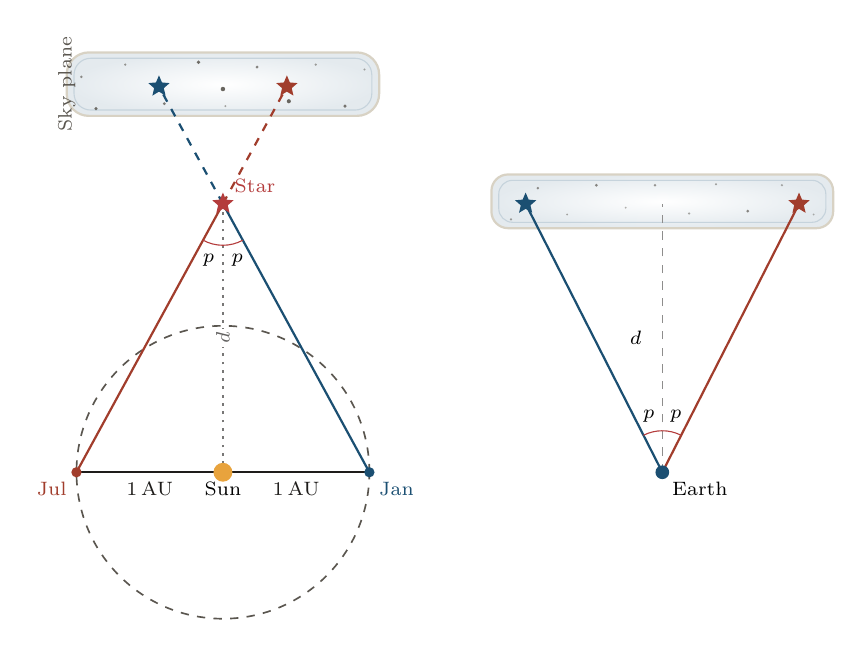
\begin{tikzpicture}[>=Stealth, scale=0.62, font=\scriptsize]

			% ================= Panel A: Sun-Earth-star geometry =================
			\begin{scope}
				\coordinate (O)  at (0,0);
				\coordinate (E1) at (3,0);
				\coordinate (E2) at (-3,0);
				\coordinate (S)  at (0,5.5);
				\coordinate (P1) at (-1.31,7.9);
				\coordinate (P2) at (1.31,7.9);

				\draw[muted, dashed, line width=0.6pt] (O) circle (3);

				\shade[
				shading=radial,
				inner color=white,
				outer color=astroblue!12,
				rounded corners=8pt
				]
				(-3.2,7.3) rectangle (3.2,8.6);

				\draw[linecol, thick, rounded corners=8pt]
				(-3.2,7.3) rectangle (3.2,8.6);

				\draw[astroblue!25, thin, rounded corners=6pt]
				(-3.05,7.42) rectangle (3.05,8.48);

				\node[muted, rotate=90] at (-3.2,7.95) {Sky plane};

				\foreach \x/\y/\r/\o in {
					-2.6/7.45/1.0pt/0.85,
					-2.0/8.35/0.7pt/0.6,
					-1.2/7.55/0.9pt/0.75,
					-0.5/8.4/1.1pt/0.85,
					0.05/7.5/0.6pt/0.5,
					0.7/8.3/0.9pt/0.7,
					1.35/7.6/1.2pt/0.9,
					1.9/8.35/0.7pt/0.55,
					2.5/7.5/1.0pt/0.8,
					2.9/8.25/0.6pt/0.5,
					-2.9/8.1/0.8pt/0.65,
					0/7.85/1.3pt/0.9
				}{
					\fill[muted, opacity=\o] (\x,\y) circle (\r);
				}

				\draw[astroblue, thick] (E1) -- (S);
				\draw[astroblue, dashed, thick] (S) -- (P1);
				\draw[accent, thick] (E2) -- (S);
				\draw[accent, dashed, thick] (S) -- (P2);

				\draw[
				ink!60,
				dash pattern=on 1pt off 2pt,
				line width=0.6pt
				]
				(O) -- (S);

				\node[
				ink!70,
				rotate=90,
				fill=white,
				inner sep=1pt
				]
				at ($(O)!0.5!(S)$) {$d$};

				\draw[ink, thick] (O) -- (E1);
				\draw[ink, thick] (O) -- (E2);

				\node[ink, below] at ($(O)!0.5!(E1)$) {$1\,\mathrm{AU}$};
				\node[ink, below] at ($(O)!0.5!(E2)$) {$1\,\mathrm{AU}$};

				\draw pic[
				"$p$",
				draw=colone,
				angle radius=15,
				angle eccentricity=1.4
				]
				{angle=O--S--E1};

				\draw pic[
				"$p$",
				draw=colone,
				angle radius=15,
				angle eccentricity=1.4
				]
				{angle=E2--S--O};

				\fill[sunyellow] (O) circle (5.5pt);
				\node[below] at (O) {Sun};

				\fill[astroblue] (E1) circle (3pt);
				\node[astroblue, below right] at (E1) {Jan};

				\fill[accent] (E2) circle (3pt);
				\node[accent, below left] at (E2) {Jul};

				\node[
				colone,
				star,
				star points=5,
				star point ratio=2.2,
				fill=colone,
				inner sep=1.3pt
				] at (S) {};

				\node[colone, above right=1pt] at (S) {Star};

				\node[
				astroblue,
				star,
				star points=5,
				star point ratio=2.2,
				fill=astroblue,
				inner sep=1.3pt
				] at (P1) {};

				\node[
				accent,
				star,
				star points=5,
				star point ratio=2.2,
				fill=accent,
				inner sep=1.3pt
				] at (P2) {};
			\end{scope}

			% ================= Panel B: Earth close-up (same scale as Panel A) =================
			\begin{scope}
				\coordinate (E)  at (9,0);
				\coordinate (S1) at (6.2,5.5); % January
				\coordinate (S2) at (11.8,5.5);  % July
				\coordinate (M)  at (9,5.5);

				\shade[
				shading=radial,
				inner color=white,
				outer color=astroblue!12,
				rounded corners=6pt
				]
				(5.5,5.0) rectangle (12.5,6.1);

				\draw[linecol, thick, rounded corners=6pt]
				(5.5,5.0) rectangle (12.5,6.1);

				\draw[astroblue!25, thin, rounded corners=5pt]
				(5.65,5.12) rectangle (12.35,5.98);

				\foreach \x/\y/\r/\o in {
					5.9/5.18/0.7pt/0.55,
					6.45/5.82/0.8pt/0.65,
					7.05/5.28/0.6pt/0.5,
					7.65/5.88/0.9pt/0.7,
					8.25/5.42/0.6pt/0.45,
					8.85/5.88/0.8pt/0.6,
					9.55/5.3/0.7pt/0.5,
					10.1/5.9/0.6pt/0.55,
					10.75/5.35/0.9pt/0.7,
					11.45/5.88/0.7pt/0.5,
					12.1/5.28/0.6pt/0.45
				}{
					\fill[muted,opacity=\o] (\x,\y) circle (\r);
				}

				\draw[astroblue, thick] (E) -- (S1);
				\draw[accent, thick] (E) -- (S2);

				\draw[
				ink!50,
				dashed,
				line width=0.6pt
				]
				(E) -- (M);

				\draw pic[
				"$p$",
				draw=colone,
				angle radius=15,
				angle eccentricity=1.4
				]
				{angle=M--E--S1};

				\draw pic[
				"$p$",
				draw=colone,
				angle radius=15,
				angle eccentricity=1.4
				]
				{angle=S2--E--M};

				\node[left=4pt] at ($(E)!0.5!(M)$) {$d$};

				\fill[astroblue] (E) circle (4pt);
				\node[below right] at (E) {Earth};

				\node[
				astroblue,
				star,
				star points=5,
				star point ratio=2.2,
				fill=astroblue,
				inner sep=1.3pt
				] at (S1) {};

				\node[
				accent,
				star,
				star points=5,
				star point ratio=2.2,
				fill=accent,
				inner sep=1.3pt
				] at (S2) {};
			\end{scope}

		\end{tikzpicture}
\end{document}
